% Re-defined by Z.C.TIAN (https://github.com/doem97)
% This version comply with the Official EEE Dissertation Guidline in [EEE dissertation] (http://www.eee.ntu.edu.sg/programmes/CurrentStudents/Graduate_Coursework/mscProg/disHome/Pages/home.aspx)
% More information about dissertation can be found in [NTU thesis](http://research.ntu.edu.sg/rieo/RI/Pages/Theses--Dissertations.aspx)
% Based on W.M.ZHAO version, original link in overleaf:
% (https://www.overleaf.com/latex/templates/ntu-master-dissertation/ngnhrrwryccv)

\documentclass[12pt]{report}
\usepackage{titlesec}
\titleformat{\chapter}
  {\normalfont\LARGE\bfseries}{\thechapter}{1em}{}
\titlespacing*{\chapter}{0pt}{2.5ex plus 0ex minus .2ex}{2.3ex plus .2ex}
\makeatletter
\renewcommand{\@makechapterhead}[1]{%
  {\noindent\raggedright\normalfont% Alignment and font reset
   \huge\bfseries \@chapapp\space\thechapter~~#1\par\nobreak}% Formatting
  \vspace{\baselineskip}% ...just a little space
}
\makeatother
%% Useful packages
\usepackage[a4paper,top=2cm,bottom=3cm,left=2cm,right=2cm,marginparwidth=1cm,headheight=10pt]{geometry}
\usepackage{amsmath}
\usepackage{cite}
\usepackage{courier}
\usepackage{minted} % For highlighted source code
\usepackage[titletoc]{appendix}
\usepackage[export]{adjustbox}
\usepackage[nottoc,notlot,notlof]{tocbibind}
\usepackage[labelfont=bf, textfont=bf]{caption}
\usepackage{graphicx}
\usepackage{hyperref}
\usepackage{float}
\usepackage{setspace}
\usepackage{subfigure}
\usepackage{setspace}
\usepackage{lipsum}
\usepackage{fancyhdr} % Fancy header
\usepackage{url}
\usepackage{tabularx}
\usepackage[utf8]{inputenc}
\usepackage{mathptmx} %Times Font
\usepackage{longtable}
%==== Header and Footer configure ====
% Define the plain pagestyle used by most chapters
\fancypagestyle{plain}{
\fancyhf{} % Clear header footer
\fancyhead[R]{\bf \textsl{\leftmark} \vspace{0.1in}}
\fancyfoot[R]{\thepage}
% Set the right side of the footer to be the page number
\renewcommand{\headrulewidth}{2pt}
}
% For those Chapter* (Can't use \leftmark to call their chapter name directly)
\fancypagestyle{addin}{
\fancyhf{} % Clear header footer
\fancyhead[R]{\bf \textsl{\leftmark} \vspace{0.1in}}
% Set the right side of the footer to be the page number
\fancyfoot[R]{\thepage}
\renewcommand{\headrulewidth}{2pt}
}

%==== Overall Config ====
\setlength{\parindent}{0in} % Set paragraph indent as 0
% \setlength{\fboxsep}{-0.3in}%
\setlength{\fboxrule}{0.5pt} % Set the bounding box around the image as 0.5pt
\pagestyle{plain}



\begin{document}
\fontdimen2\font=0.5em% inter word space
%==== FRONT PART====
\begin{titlepage}

\begin{figure}[h!]
\centering

\includegraphics[width=1\textwidth]{Title/NTU_logo.png}
\caption*{}
\label{fig:entropy} 
\end{figure}

\vspace{1.5in}

\centering
\Huge{\textbf{CZ4013 Distributed System\\Assignment}}\\[1.5in]

\footnotesize
\begin{longtable}{|l|l|}
\hline
Zhang Yongzhe                       & Yang Yubei               \\ \hline
\endhead
%
Client: Service1,2,3,4,5,6          & Server: Service1,2,3,5,6 \\ \hline
Server: Service4                    & Design UDP Communication \\ \hline
Design Message Structure            &                          \\ \hline
Implement Invocation Semantics      &                          \\ \hline
Conduct fault-tolerance Experiments &                          \\ \hline
\caption{Contribution}
\end{longtable}

\normalsize{\textbf{SCHOOL OF COMPUTERSCIENCE AND ENGINEERING}}\\[0.2in]

% \textbf{A DISSERTATION SUBMITTED IN PARTIAL FULFILMENT OF\\
% THE REQUIREMENTS FOR THE DEGREE OF\\
% MASTER OF SCIENCE IN DIGITAL MEDIA TECHNOLOGY}\\[0.25in]

\large{\textbf{2021}}
\end{titlepage}
\newpage % Coverpage
\include{Title/titlepage} % Titlepage

%\begingroup
%\let\cleardoublepage\clearpage

\pagenumbering{roman}

\renewcommand*\contentsname{\centering Table of Contents}
\tableofcontents
\newpage



%\endgroup

%==== MAIN PART ====

\pagenumbering{arabic}
%=== CHAPTER TWO (2) ===
%=== Literature Review ===

\chapter{Introduction}
\begin{spacing}{1}
\setlength{\parskip}{0in}

This project consolidates the basic knowledge about interprocess communication and remote invocation by constructing client and server programs that use UDP as the transport protocol. A distributed facility booking system based on client-server architecture is implemented. The server program stores the information of facilities and booking information, and provides different services,  including query, book, change booking,cancel booking and monitoring, which can be remote access by clients. The client program provides an interface for users to invoke these services.

\section{Environment}

The following are the necessary environment to run the system.
Operating System: The facility booking system is developed and tested in a GNU/Linux environment.
Programming Language: Java.


\section{Assumption}
Several assumptions have been made in developing the system as follows:
\begin{enumerate}
   \item General Assumptions:
   \begin{itemize}
      \item Client-Server Communication: All clients are assumed to know IP address and port number.
      \item Request Concurrency: Server and client handle the user input in sequential order. 
   \end{itemize}
   \item Client Assumptions:
      \begin{itemize}
      \item User Interface: The user interaction to the system is solely done in the command-line interface.
      \item User Input: There are minimum error checking (e.g. Variable Type checking). 
   \end{itemize}
    \item Facility Assumptions:
        \begin{itemize}
      \item Four different facilities of 2 types are provided: LT1, LT2, MR1, MR2.
      \item Facility Timetable: (8:00am - 6:00pm, interval: 1h, total: 10 intervals)
   \end{itemize}
    \item Server Assumptions:
        \begin{itemize}
      \item Server1 Query
        \begin{itemize}
            \item A user can only query availability of a service within 7 days.
        \end{itemize}
      \item Server2 Booking
      \begin{itemize}
          \item  A user can only book a facility one day advance. (e.g. Today is Apr 1st. Can only book from Apr 2nd.)
          \item A user can book a facility either 1 hour or 2 hours each time.
      \end{itemize}
        \item Server3 Change Booking Time
        \begin{itemize}
            \item A user can only change booking time to other slots of the same day.
        \end{itemize}
        \item Server5 Auto-Booking
        \begin{itemize}
            \item A user can only choose the type of facility. 
            \item Server will return the nearest available slots in 2 facilities of the required type.
            \item If there are no available slots for the next day in both 2 facilities, the booking is unsuccessful.
        \end{itemize}
        \item Server6 Cancel Booking
        \begin{itemize}
            \item Once the booking is canceled, it cannot be restored.
        \end{itemize}
   \end{itemize}
   
\end{enumerate}




%=== END OF CHAPTER TWO ===
\end{spacing}
\newpage

%=== CHAPTER THREE (3) ===
%=== (Actual work done and contribution, including literature survey) ===

\chapter{Design}
\begin{spacing}{1}
\setlength{\parskip}{0in}
%  (Actual work done and contribution, including literature survey)


\section{Architecture Design}

We applied ECB design pattern on the structure of our program. Specifically, the client and server are classified in to 3 layers, which are entity, control and boundary.

\section{Communication Design}
\subsection{Message Format}
On the client side, we designed two types of messages, which are Request and Acknowledgement. And the request message is divided into 4 sections: message type, Message ID, Service ID, data shown in Table 2.1. And the usage of different sections are described in the below:
\begin{enumerate}
  \item Message Type: An integer (0 or 1), which is used by the server to differentiate a message is a Request or Acknowledgement. If the value is 1, it indicates as a request message.
  \item Message ID: An integer, which is used by the server to filter duplicated request messages by checking a hash table storing previous processed requests, when the At-Most-Once invocation is enabled.
  \item Service ID: An integer, which is used by the server to dispatch the request to a corresponding service handler.
  \item Data: See the Common Data Representation.
\end{enumerate}
\begin{table}[h!]
\centering
\begin{tabular}{|l|l|l|l|}
\hline
Msg Type & Msg ID & Service ID & Data \\ \hline
\end{tabular}
\caption{Request Message}
\end{table}

The Acknowledgement is divided into 2 sections: message type and status as shown in Table 2.2. And the usage of different sections are described in the below:
\begin{enumerate}
    \item Message type: An integer (0 or 1), which is used by the server to differentiate a message is a Request or Acknowledgement. If the value of the message type is 0, it indicates as an acknowledgement message. 
    \item Status: An integer (0 or 1), which is used by the client to acknowledge whether it receives the response from server successfully (1) or not (0) within a timeout period (controlled by Param MAXTIMEOUTCOUNT and UDPTIMEOUT).
\end{enumerate}

\begin{table}[h!]
\centering
\begin{tabular}{|l|l|l|l|}
\hline
Msg Type & Msg ID & Status \\ \hline
\end{tabular}
\caption{Acknowledgement Message}
\end{table}


On the server side, to improve the efficiency and better use of available channel bandwidth, we piggybacked the acknowledgement on the response message. And the response message is divided into 3 sections: ACK Status, Processed Status, Data as shown in Table 2.3. And the usage of different sections are described in the below:
\begin{enumerate}
    \item ACK status: An integer (0 or 1), the piggybacked acknowledgement is used to indicate whether the server receives the request from client successfully (1) or not (0).
    \item Processed status: An integer (0 or 1), which is used by client to tell whether the request is processed by server successfully(1) or not(0). Client will invoke different functions to display correct or error messages.
    \item Data: See the Common Data Representation.
\end{enumerate}

\begin{table}[h!]
\centering
\begin{tabular}{|l|l|l|l|}
\hline
ACK Status(Piggyback) & Processed Status & Data \\ \hline
\end{tabular}
\caption{Response Message}
\end{table}


\subsection{Marshal / Unmarshal}
\begin{enumerate}
    \item Primitive Type: int.
Marshalling an integer into a byte array of size 4. To obtain the $i$th byte in the array, we can right shift the int by 8 * (4 - i) number of times.
		Unmarshalling the byte array back to an int can be left shifted the $i$th byte in the array  by 8 * (4 - i) number of times, and then perform OR  operation.
    \item Non-primitive Type: String.
Marshalling/unmarshalling a String depends on the number of characters. Each byte represents one character of a String.
\end{enumerate}

\subsection{The Common Data Representation}
\begin{enumerate}
    \item The Big-Endian ordering is used when we marshal/unmarshal data.
    \item We assumed that the client and server have common knowledge of the order and types of the variables in the data section.
    \item A data session contains different variables depends on the service ID.  We inserted the length of a variable followed by that variable shown in Table 2.4.
\end{enumerate}
\begin{table}[h!]
\centering
\begin{tabular}{|l|l|l|l|l|}
\hline
len1 & var1 & len2 & var2 & ... \\ \hline
\end{tabular}
\caption{Data Section}
\end{table}

%=== END OF CHAPTER THREE ===
\end{spacing}


%=== CHAPTER FOUR (4) ===
%=== Test and Experiments ===

\chapter{Services}
\begin{spacing}{1}

\section{Service1: Query Facility Availability}
The request and response message has the following format shown in Table 3.1.\\
This service allows users to query the availability of a facility in the next 7 days. Client needs to provide facility name(e.g. LT1) and number of days he wants to query. Service1 will return a response with available intervals of the required facility within required days.
Requests will always be processed correctly, so there is no fail case for this service and response status = 1.

\begin{table}[h!]
\centering
\begin{tabular}{|l|l|l|l|l|}
\hline
\multicolumn{5}{|c|}{Service1: Query Facility Availability} \\ \hline
\multicolumn{2}{|l|}{\textbf{Request}} & ReadIn Syntax Check & \multicolumn{2}{l|}{\textbf{Response}} \\ \hline
\textbf{Facility Name} & String & Facility name exists. & \textbf{Available intervals} & String \\ \hline
\textbf{\# of Days} & Int {[}1,7{]} & Number of days in range {[}1-7{]}. &  &  \\ \hline
\end{tabular}
\caption{Service1}
\end{table}

\section{Service2: Book a facility}
The request and response message has the following format shown in Table 3.2.\\
This service allows users to book a facility. Client needs to provide facility name, date to book, slot starting time and ending time. Service2 will return booking information if there is no collision, or return error information if there is collision. Specifically, in success case(1), server response status =1. In the unsuccessful case(2,3,4), server response status = 0.
A BookingInfo String contains the following information. (e.g.”01-20210322-LT1-1113-1511”)

\begin{table}[h!]
\centering
\begin{tabular}{|l|l|l|l|l|l|}
\hline
\multicolumn{6}{|c|}{Service2: Book a facility} \\ \hline
\multicolumn{2}{|l|}{\textbf{Request}} & ReadIn Syntax Check & \multicolumn{2}{l|}{\textbf{Response}} & Case Comment \\ \hline
\textbf{Facility Name} & String & Facility name exists. & \textbf{BookingInfo} & String & (1) Success \\ \hline
\textbf{Date} & String & \begin{tabular}[c]{@{}l@{}}Date in correct \\ String format.\\ Date in range \\ {[}next day \\ to one week{]}.\end{tabular} & \textbf{Complete collision} & String & (2) Unsuccess \\ \hline
\textbf{Start time} & int & In range {[}8-18{]} & \textbf{Partial Collision(1)} & String & (3) Unsuccess \\ \hline
\textbf{End time} & int & In range {[}8-18{]} & \textbf{Partial Collision(2)} & String & (4) Unsuccess \\ \hline
\end{tabular}
\caption{Service2}
\end{table}

\section{Service3: Change booking time}
The request and response message has the following format shown in Table 3.3.\\
This service allows users to change the previously booked facility to another time slot within the same day. Client needs to provide BookingID and the offset he wants to change. Service3 will check if the BookingID exists, the offset makes timeslot out of 8am-6pm bound, or the intended change slot has collision with other booked slots.  If all requirements are met, Service3 will return a new BookingInfo. Else, corresponding error messages are returned.
Specifically, in success case(1), server response status =1. In the unsuccessful case(2,3,4), server response status = 0.

\begin{table}[h!]
\centering
\begin{tabular}{|l|l|l|l|l|l|}
\hline
\multicolumn{6}{|c|}{Service3: Change booking time} \\ \hline
\textbf{Request} &  & ReadIn Syntax Check & \multicolumn{2}{l|}{\textbf{Response}} & Case Commen \\ \hline
\textbf{Booking ID} & int & Positive Int & \textbf{BookingInfo} & String & (1) Success \\ \hline
\textbf{Offset of change} & int & Positive/ Negative Int & \textbf{BookingID not found} & String & (2) Unsuccess \\ \hline
 &  &  & \textbf{Offset outof bound} & String & (3) Unsuccess \\ \hline
 &  &  & \textbf{Change has collision} & String & (4) Unsuccess \\ \hline
\end{tabular}
\caption{Service3}
\end{table}

\section{Service4: Monitor}
The request and response message has the following format shown in Table 3.4.\\
This service allows users to monitor the availability of a facility over the week. Users can indicate the facility and duration that they want to monitor on the client side. The server will register each client when receive the monitoring requests. And then, when a facility has a new booking, change or cancel, the server will notify the clients which are registering under this facility by using callback mechanism.

\begin{table}[h!]
\centering
\begin{tabular}{|l|l|l|l|l|}
\hline
\multicolumn{5}{|c|}{Service4: Monitor} \\ \hline
\multicolumn{2}{|l|}{\textbf{Request}} & ReadIn Syntax Check & \multicolumn{2}{l|}{\textbf{Response}} \\ \hline
\textbf{Facility Name} & String & Facility name exists. & \textbf{Available intervals in 7 days} & String \\ \hline
\textbf{Duration(in second)} & Int & Positive Int  &  & \\ \hline
\end{tabular}
\caption{Service4}
\end{table}

\section{Service5: Auto booking facility}
The request and response message has the following format shown in Table 3.5.\\
This service will auto select a facility with one hour which is the most recent available for the user. Client needs to provide facility type. Service5 will check if there are any left available slots of the required facility type on the next day. If there is, return the most recent available slot of 2 facilities.  Else, return an error message.
Specifically, in success case(1), server response status =1. In the unsuccessful case(2), server response status = 0.


\begin{table}[H]
\centering
\begin{tabular}{|l|l|l|l|l|l|}
\hline
\multicolumn{6}{|c|}{Service5(Non-idempotent): Auto booking facility} \\ \hline
\multicolumn{2}{|l|}{\textbf{Request}} & Comment & \multicolumn{2}{l|}{\textbf{Response}} & Case Comment \\ \hline
\textbf{Facility Type} & int & \begin{tabular}[c]{@{}l@{}}1: Lecture theater\\ 2: Meeting room\end{tabular} & \textbf{BookingInfo} & String & (1)Success \\ \hline
 &  &  & \textbf{No Available Slot} & String & (2)Unsuccess \\ \hline
\end{tabular}
\caption{Service5}
\end{table}

\section{Service6: Cancel Booking}
The request and response message has the following format shown in Table 3.6.\\
This service allows users to cancel a previous booking. Client needs to provide the Booking ID which is received in Service2 or Service3. Service6 will check if this Booking ID exists. If it exists, return a successful cancellation message to the client. Else, return an error message.
Specifically, in success case(1), server response status =1. In the unsuccessful case(2), server response status = 0.

\begin{table}[h!]
\centering
\begin{tabular}{|l|l|l|l|l|}
\hline
\multicolumn{5}{|c|}{Service6(Idempotent): Cancel Booking} \\ \hline
\multicolumn{2}{|l|}{\textbf{Request}} & \multicolumn{2}{l|}{\textbf{Response}} & Case Comment \\ \hline
\textbf{Booking ID} & int & \textbf{ChangeInfo} & String & (1)Success \\ \hline
 &  & \textbf{BookingID not found} & String & (2)Unsuccess \\ \hline
\end{tabular}
\caption{Service6}
\end{table}
%=== END OF CHAPTER FOUR ===
\end{spacing}
\newpage

%=== CHAPTER FIVE (5) ===
%=== Discussion ===
\chapter{Fault Tolerance}
\begin{spacing}{1}
\setlength{\parskip}{0in}

\section{Design Ideas}

The UDP transport protocol is naively designed for low latency but not fault-tolerant transmission. UDP has no handshaking mechanism to guarantee reliable connections between clients and servers as compared to TCP. We implemented some techniques such as time-out, retransmit requests/responses, maintain histories and filter duplicated requests to guarantee the system to be fault-tolerant to message loss. 
Firstly, we design a three-way handshaking communication between servers and clients. When the server receives the response from clients, it processes the request and sends a response message piggybacking ACK to the client. At last, clients will send a ACK message to acknowledge whether it received the response successfully or not.\\

\begin{figure}[h!]
    \centering
  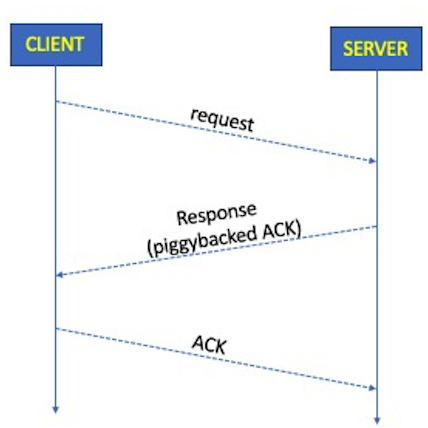
\includegraphics[width=6cm, height=6cm]{Image/4.png}
  \caption{Design}
\end{figure}

We considered three scenarios of message loss during transmission between server and client.
\subsection{Scenario 1: Request Loss}
This scenario is analyzed based on the assumption of Response and Acknowledgement are never lost.
As shown in Figure 4.2, to detect the request loss, we implemented a timeout mechanism on the client side. If a client doesn’t receive any replies from the server after a certain time, the client will send an acknowledgement message with status 0 (NAK). When the server receives a NAK message from the client, it will send a piggybacked NAK back to the client, So, the client will resend the request. This process keeps repeating until the client receives a piggybacked ACK message from the server.

\begin{figure}[h!]
\centering
  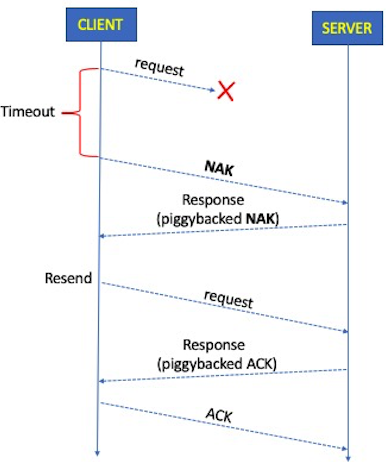
\includegraphics[width=6cm, height=6cm]{Image/2.png}
  \caption{Request Lost}
\end{figure}


\subsection{Scenario 2: Response Loss}
This scenario is analyzed based on the assumption of Request and Acknowledgement are never lost.
We also used the timeout mechanism on the client side to detect the response message loss during transmission. As shown in Figure 4.3, the differences with the scenario 1 is after the server (if enable At-Most-Once) receives a NAK message from client, the server will first get the message ID from the NAK message (more detailed in the Message Structure) , and then search in a maintained Hashtable with the messageID to check whether a previous processed request with the same message ID can be found.
If found, the server just resend the response message with piggybacking ACK. If not found, the server will just send a NAK back to the client (At-Least-Once just simply sends a NAK without searching in the Hashtable).


\begin{figure}[h!]
\centering
  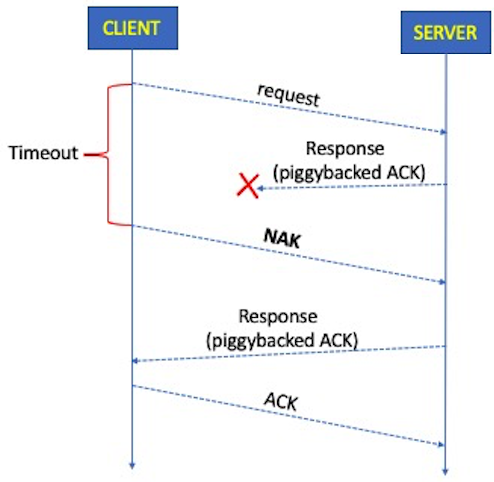
\includegraphics[width=6cm, height=6cm]{Image/1.png}
  \caption{Response Lost}
\end{figure}


\subsection{Senario 3: Acknowledgment Loss}
This scenario is analyzed based on the assumption of response and request are never lost. As shown in Figure 4.4, 
The purpose of the Acknowledgement is to acknowledge the client has successfully received the reply from the server or not. After receiving an ACK from client, server can remove the previous record in the Hashtable(if enable At-Most-Once). So, if the acknowledgment message is lost, the Hashtable storing previous processed records will never be removed. So, our proposed solution for this issue is to implement a timeout mechanism on the server side to auto remove a previous record within a certain time to avoid the Hashtable keeps growing. But, from the experience, the loss of an acknowledgement message won’t cause any operations to produce unexpected results.

\begin{figure}[h!]
\centering
  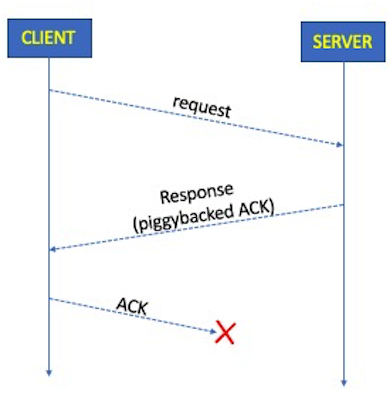
\includegraphics[width=6cm, height=5cm]{Image/3.png}
  \caption{Acknowledge Lost}
\end{figure}



\section{Experiments}

\subsection{Non-Idempotent}
We use our Service 5 (Auto-booking function) to conduct the three message lost scenarios with two different invocation semantics under the failure rate is 50\%. As shown in Table 4.1, we verified that the At-Least-Once semantics will invoke multiple times of bookings with randomly picking up the latest available slots on the server side under the response-loss scenario only.

\begin{table}[!h]
\centering
\begin{tabular}{|l|l|l|}
\hline
 & At-Least-Once & At-Most-Once \\ \hline
Request loss & \begin{tabular}[c]{@{}l@{}}Auto select one \\ latest available slots\end{tabular} & Auto select one latest available slots \\ \hline
Response loss & \begin{tabular}[c]{@{}l@{}}(\textbf{Unexpected})Auto select \\\textbf{multiple} latest available slots\end{tabular} & Auto select one latest available slots \\ \hline
Acknowledgement loss & \begin{tabular}[c]{@{}l@{}}Auto select one \\ latest available slots\end{tabular} & Auto select one latest available slots \\ \hline
\end{tabular}
\caption{Non-Idempotent}
\end{table}

\subsection{Idempotent}
We use our Service 6 (cancel bookings) to conduct the three message lost scenarios with two different invocation semantics under the failure rate is 50\%. As shown in Table 4.2, We verified that all the scenarios can produce correct operational results regarding of the invocation semantics.
\begin{table}[H]
\centering
\begin{tabular}{|l|l|l|}
\hline
 & At-Least-Once & At-Most-Once \\ \hline
Request loss & Booking is cancelled successfully & \begin{tabular}[c]{@{}l@{}} Booking is cancelled \\successfully\end{tabular} \\ \hline
Response loss &\begin{tabular}[c]{@{}l@{}} Booking is cancelled successfully(server)\\ (Booking ID is not found,client) \end{tabular} &\begin{tabular}[c]{@{}l@{}} Booking is cancelled \\successfully\end{tabular}  \\ \hline
Acknowledgement loss & Booking is cancelled successfully & \begin{tabular}[c]{@{}l@{}} Booking is cancelled \\successfully\end{tabular} \\ \hline
\end{tabular}
\caption{Idempotent}
\end{table}
\\

\chapter{Conclusion}
We designed and implemented a distributed booking system fault-tolerating to the message loss during transmission with UDP protocol.
We analysed and experimented three different message loss scenarios and implemented several mechanisms including timeout, re-transmit request/response messages, filter duplicated requests. Finally, we compared two different invocation semantics under three different message loss scenarios and found that the non-idempotent
operations could produce wrong results when applied At-Least-Once semantic under the response-loss scenario.

%=== END OF CHAPTER FIVE ===
\end{spacing}
\include{Chapter5/Chapter5}
\include{Chapter6/Chapter6}
%==== ENDING PART ===

\renewcommand\bibname{References}
\bibliographystyle{unsrt}
\begin{spacing}{0.5}
\bibliography{Ref/References}
\end{spacing}
\newpage

\include{Appendix/appendix}
%==== END OF ALL ===
\end{document}
